
\documentclass{sigplanconf}

% The following \documentclass options may be useful:

% preprint      Remove this option only once the paper is in final form.
% 10pt          To set in 10-point type instead of 9-point.
% 11pt          To set in 11-point type instead of 9-point.
% authoryear    To obtain author/year citation style instead of numeric.
\synctex=-1

\usepackage[utf8]{inputenc}
\usepackage{array}
\usepackage{color}
\usepackage{amsmath}
\usepackage{amssymb}
\usepackage{fixltx2e}
\usepackage{graphicx}
\usepackage[unicode=true,pdfusetitle,
 bookmarks=true,bookmarksnumbered=false,bookmarksopen=false,
 breaklinks=false,pdfborder={0 0 1},backref=false,colorlinks=false]{hyperref}


\makeatletter
\usepackage{enumitem}
\usepackage{multicol}
\usepackage{tabularx}

%%%%%%%%%%%%%%%%%%%%%%%%%%%%%% LyX specific LaTeX commands.
\usepackage{float}
\floatstyle{ruled}
\newfloat{code}{tbp}{loa}
\providecommand{\codename}{Listing}
\floatname{code}{\protect\codename}



% nice listings
\usepackage{xcolor}
\usepackage{newverbs}

\usepackage{color}
\definecolor{verylightgray}{rgb}{0.93,0.93,0.93}
\definecolor{darkblue}{rgb}{0.2,0.2,0.6}
\definecolor{commentgreen}{rgb}{0.25,0.5,0.37}
\usepackage{letltxmacro}

\usepackage{listings}

\makeatletter
\LetLtxMacro{\oldlstinline}{\lstinline}

\renewcommand\lstinline[1][]{%
  \Collectverb{\@@myverb}%
}

\def\@@myverb#1{%
    \begingroup
    \fboxsep=0.2em
    \colorbox{verylightgray}{\oldlstinline|#1|}%
    \endgroup
}
\makeatother




\lstset{backgroundcolor={\color{verylightgray}},
  basicstyle={\scriptsize\ttfamily},
  commentstyle={\ttfamily\color{commentgreen}},
  keywordstyle={\bfseries\color{darkblue}},
  morecomment={[l]{//}},
  tabsize=4,
  morekeywords={foreach,in,def,type,dynamic,Int,
    Boolean,infer,void,super,if,boolean,int,else,
    while,do,extends,class,assert,for,switch,case,
    private,protected,public,const,final,static,
    interface,new,true,false,null,return}}
\renewcommand{\lstlistingname}{Listing}

% Keine "Schusterjungen"
\clubpenalty = 10000
% Keine "Hurenkinder"
\widowpenalty = 10000 \displaywidowpenalty = 10000


% \newcommand{\mynote}[2]{%
%   \textcolor{red}{%
%     \fbox{\bfseries\sffamily\scriptsize#1}%
%     {\small$\blacktriangleright$\textsf{\emph{#2}}$\blacktriangleleft$}%
%   }%
% }

% \newcommand\remi[1]{\mynote{Remi}{#1}}
% \newcommand\cfbolz[1]{\mynote{cfbolz}{#1}}
% \newcommand\arigo[1]{\mynote{arigo}{#1}}

% \newcommand{\comment}[1]{}


\begin{document}

\special{papersize=8.5in,11in}
\setlength{\pdfpageheight}{\paperheight}
\setlength{\pdfpagewidth}{\paperwidth}

\conferenceinfo{DLS 2014}{to be supplied}
\copyrightyear{2014}
%\copyrightdata{978-1-nnnn-nnnn-n/yy/mm}
\doi{nnnnnnn.nnnnnnn}

% Uncomment one of the following two, if you are not going for the
% traditional copyright transfer agreement.

%\exclusivelicense                % ACM gets exclusive license to publish,
                                  % you retain copyright

%\permissiontopublish             % ACM gets nonexclusive license to publish
                                  % (paid open-access papers,
                                  % short abstracts)

%% \titlebanner{banner above paper title}        % These are ignored unless
%% \preprintfooter{short description of paper}   % 'preprint' option specified.

\title{A Transactional Memory System for Parallel Python}
%\subtitle{DLS'14}

% \comment{
% A Platform for Parallelism in Dynamic languages
% Parallelism for Python
% A TM Implementation for Python
% Transactional Memory as a foundation for parallel Python
% Transactional Memory as a foundation for parallelism in Python
% Parallel Python based on VM-assisted TM
% Parallel Python based on VM-assisted Transactional Memory
% A Platform for parallel Python
% A TM Platform for parallel Python
% A Transactional Memory Platform for parallel Python
% A Transactional Memory system for parallel Python

% Virtual Memory Assisted Transactional Memory for Dynamic Languages}

\authorinfo{Remigius Meier}
           {Department of Computer Science\\ ETH Zürich, Switzerland}
           {remi.meier@inf.ethz.ch}
\authorinfo{Armin Rigo}
           {www.pypy.org}
           {arigo@tunes.org}
\authorinfo{Thomas Gross}
           {Department of Computer Science\\ ETH Zürich, Switzerland}
           {thomas.gross@inf.ethz.ch}

\maketitle

\begin{abstract}

Since some years, the popularity of dynamic languages is on the rise.
A common trait of many of these language's implementations is the use of
a single global interpreter lock (GIL) to synchronise the interpreter
in a multithreading scenario. Since this lock effectively serialises
the execution, applications can not make use of the increasing parallelism in
current hardware.

In this paper, we present a software transactional memory (STM) system
specifically designed for the purpose of replacing the GIL in dynamic
language interpreters while keeping the semantics. The key idea is a
close integration of STM with the garbage collector to approach
atomicity, synchronisation, and memory management in a unified
way. Additionally, we implement atomic blocks as a scalable
synchronisation mechanism by exposing part of this STM system to
applications.

The described system uses a combination of features present in current
CPUs, so that the parallelisation benefits outweigh the system's
overhead already on 2 threads when comparing two Python interpreters
-- one with STM and one with a GIL.


\end{abstract}

%\category{CR-number}{subcategory}{third-level}

% general terms are not compulsory anymore,
% you may leave them out
%% \terms
%% term1, term2

\keywords
transactional memory, global interpreter lock, dynamic language,
python, virtual machine


\section{Introduction}


Dynamic languages like Python, PHP, Ruby, and JavaScript receive a lot
of attention but have not yet embraced parallelism. A parallel
programming model was not part of the design of those languages. Thus,
the reference implementations of, e.g., Python and Ruby use a single,
global interpreter lock (GIL) to serialise the execution of code in
threads. The use of a single global lock causes several disadvantages,
and as multi-core processors become the de facto standard in platforms
ranging from smart phones to data centres, the issue of parallel
execution must be addressed by these dynamic languages.

Unfortunately the GIL plays a central role in current
implementations. Even recent efforts to address the performance problems
of dynamic languages with just-in-time compilers (JIT)
(e.g., PyPy~\cite{cfbolz09}, V8~\cite{kevin10},
IonMonkey~\cite{ionmonkey}) keep the GIL; Jython (an
implementation of Python that is based on the JVM) is a notable
exception.

The standard model employed in these systems is fairly
straightforward: there can be multiple threads, but each acquires the
GIL, then performs one (or several) instruction, and subsequently releases the
lock.  While this setup limits the benefits due to parallelism,
the use of a GIL also provides
some crucial guarantees. Since this lock is always acquired while
executing bytecode instructions and may be released only in-between
such instructions, the GIL ensures perfect isolation between multiple
threads for a series of instructions -- executing them atomically.
In addition, the GIL provides the application with a sequential
consistency model~\cite{lamport79}.

A global interpreter lock assures the atomic execution of individual
instructions but offers the programmer no help in managing concurrent
data structures. Many parallel programs must maintain invariants
involving multiple objects (or multiple fields of a single
object).  So to enable Python programs for parallel execution, we need
a way to identify which blocks of data must be executed atomically and
hardware or software support to effect this atomic execution.
This is traditionally done with locks.

\emph{Atomic blocks}~\cite{tim03,tim05} allow languages to
indicate the units of computation that must be executed atomically to
ensure correct concurrent execution.  Atomic blocks map nicely to
transactional memory, which in turn provides a convenient mechanism to replace
the GIL.  Using transactions to enclose multiple bytecode
instructions, we can get the very same semantics as provided by the
GIL while possibly executing several transactions in parallel. And by
exposing these interpreter-level transactions to the application, we
avoid the well-known problems caused by locks as applications use
atomic blocks instead of explicit acquire/release operations on
locks~\cite{christopher10,victor11,shan08}.

There have been several attempts at replacing the GIL with
TM~\cite{nicholas06,odaira14,fuad10}.  We focus here on software based
transactional memory (STM) because that provides the unique
opportunity to consider the issues of atomicity, synchronisation, and
memory management (resp. garbage collection) together.  STM systems
impose no a-priori bound on the size of an atomic block and provide
therefore a flexibility that is absent from current hardware-based TM
systems~\cite{wayforward14}.  The downside of STM systems is runtime
overhead~\cite{cascaval08,drago11}, which can be substantial despite
recent efforts to lower it~\cite{warmhoff13,spear09}.  In
this paper, we describe how we manage to lower the overhead of an STM
system so that it can serve as a viable replacement for the GIL by
leveraging the demands of a dynamic language like Python to integrate
the STM system with the garbage collector.


This paper makes the following contributions:
%\vspace{-\topsep}               % XXX:HACK:TODO
\begin{itemize}
\item We introduce a new STM system that performs well for dynamic
  language interpreters.
\vspace{3mm}               % XXX:HACK:TODO
\item We integrate the system closely with a garbage collector
  (GC) to lower the overhead of STM.
\item This new STM system is used to replace the GIL in one
  implementation of Python and is then evaluated.
\end{itemize}

The STM described here is efficient and has low overhead and is
therefore beneficial also for environments with a small number of
threads or cores.

\subsection{Application View}

We implement and evaluate our system for the Python language. Python
is a dynamic programming language that was originally designed without
concurrency in mind.
Its reference implementation, CPython~\cite{cpython}, uses a
GIL. Over the years, Python added multiple ways to provide concurrency and
parallelism to its applications. We want to highlight two of them,
namely \emph{threading} and \emph{multiprocessing}.

\emph{Threading} employs operating system (OS) threads to provide
concurrency. It is, however, limited by the GIL and thus does not
provide parallelism\footnote{At this point we should mention that it is indeed
possible to run external functions written in C instead of Python in
parallel. Our work focuses on Python itself and ignores this aspect as
it requires writing in a different language.}.  Moreover, the GIL can
only ensure correctness of the interpreter itself: applications are
required to coordinate concurrent accesses to data structures using
conventional methods -- locks being the most common way.

The second approach, \emph{multiprocessing}, uses multiple instances
of the interpreter itself and runs them in separate OS processes.
Here we actually get parallelism because there is one GIL per
interpreter, but of course we have the overhead of multiple processes~/
interpreters and also need to exchange data between them explicitly
and expensively.

We focus on the \emph{threading} approach. This requires us to remove
the GIL from the interpreter to run code in parallel on multiple
threads. One approach to this is fine-grained locking instead of a
single global lock. Jython~\cite{webjython} and
IronPython~\cite{ironpython} follow this approach. Fine-grained
locking is, however, not a \emph{direct} replacement for the GIL. It
requires multiple locks in multiple places, not only in a central
location. We on the other hand follow the direct approach of using TM
instead of the GIL. There, GIL acquisition and release operations
conceptually directly map to starting and committing transactions.

TM also allows us to attack the issue of application-level
synchronisation and atomicity. We introduce atomic blocks to the
Python language by mapping them directly to the underlying
transactions -- providing the application with the guarantees of
atomicity and isolation for the enclosed instructions.


\section{Transactional Memory Model}

In this section, we characterise the model of our TM system and its
guarantees as well as some of the design choices we made. This should
clarify the general semantics in commonly used terms from the
literature~\cite{harris10}.

The described TM system is fully implemented in software. However, we exploit
some more advanced features of current CPUs, particularly \emph{memory
segmentation, virtual memory,} and the 64-bit address space. Still,
it cannot be classified as a hybrid TM system since it currently
makes no use of any hardware TM (HTM) present in the CPU.

\subsection{Conflict Handling}

We implement an object-based TM system, thus it makes sense to detect
conflicts with \emph{object granularity}. With this choice, if two
transactions access the same object and at least one access is a
write, we count it as a conflict. Conceptually, it is based on
\emph{read} and \emph{write sets} of transactions. Reading from an
object adds the object to the read set, writing to it adds it to both
sets. Two transactions conflict if they have accessed a common object
that is in the write set of at least one of them.

The detection, or \emph{concurrency control}, works partly
\emph{optimistically} for reading objects. Read-write conflicts
between two transactions are detected in both exactly at the time when
the writing one commits. For write-write conflicts we are currently
\emph{pessimistic}: Only one transaction may have a certain object in
its write set at any point in time, others trying to write to it will
have to wait or abort. This decision needs to be evaluated further
in the future.

When a conflict is detected, we perform some simple contention
management that generally prefers the older transaction to the younger.
This gives long transactions a better chance to succeed.

\subsection{Semantics}

As required for TM systems, we guarantee complete \emph{isolation} and
\emph{atomicity} for transactions at all times. Our method of choice
is \emph{lazy version management}. Modifications by a transaction are
not visible to another transaction before the former commits.
Furthermore, the isolation provides full
\emph{opacity}~\cite{guerraoui08} to always guarantee a consistent
read set even for non-committed transactions.

To also support these properties for irreversible operations that
cannot be undone when we abort a transaction (e.g.\ I/O, syscalls, and
non-transactional code in general), we use \emph{irrevocable} or
\emph{inevitable transactions}~\cite{blundell06,spear08}. These transactions are always
guaranteed to commit, which is why they always have to win in case
there is a conflict with another, normal transaction. There is always
at most one such transaction running in the system, thus their
execution is serialised. With this guarantee, providing \emph{strong
isolation} and \emph{serialisability} between non-transactional code
is possible by making the current transaction inevitable right before
running irreversible operations.



\section{High-Level Overview}

In this section, we will present the general idea of how the TM model is
implemented.  The later section~\ref{sub:Low-level-Implementation} will
discuss it with more technical details.

\subsection{Memory Segmentation and Page Sharing}

Our STM system fundamentally builds on threads. Transactions run in
their context, and there can be only one transaction per thread at a
time. Transactions run in parallel because these threads can run in
parallel. To isolate transactions from each other, we look
at isolating the memory accesses from threads.

A naive approach to providing this complete isolation between threads
is to partition the virtual memory of a process into $N$ segments, one
for each thread currently executing.  Each segment then holds a
complete copy of the memory logically seen by the program.  All
threads read and write data inside their own segment; and this data
gets copied to other segments in an atomic fashion only when a
transaction commits.  So far, this is a model that would also work for
distributed transactional memory.

Clearly, if we are in a shared-memory setting, this model is extremely
wasteful: at any given time, most objects are identical in all, or
most, segments.  They differ only in segments that have modified but
not yet committed these objects.  So we make use of the Memory
Management Unit (MMU) of the CPU.  The MMU maps pages of virtual to
physical memory.  By changing this page mapping at the coarse unit of
one page of memory (4096 bytes), we can share memory that would
otherwise exist as identical copies in all segments.

In the common case, where objects are identical in all segments, we
can thus make these pages \emph{shared}. Conversely, when one thread~/
segment wants to modify an object, all pages of this object need to be
\emph{privatised} for this segment. This involves duplicating the
pages and changing the page mapping so that the private pages are only
accessible by this segment and full isolation is guaranteed.  This
process is illustrated in Figure~\ref{fig:Page-Remapping}.

The result is that the virtual address space of the process is bloated
by a factor $N$ -- but the real, physical memory usage is not, because most
pages are shared with their identical copies in other segments.

\begin{figure}[h]
  \centering
  \includegraphics[width=1\columnwidth]{\string"page remapping\string".pdf}
  \caption{Page Remapping: (I) initial setting. (II) remap all pages to
    segment~0, fully shared memory configuration. (III) privatise single
    pages.\label{fig:Page-Remapping}}
\end{figure}


\subsection{Memory Segmentation on x86 CPUs}

When we store into our objects the references to other objects, we
need to be careful: addresses that are valid in one segment are not
valid in another, because they would break isolation by possibly pointing to
the copy of the object in another segment.  Consequently, we would
need to adapt these addresses to the segment they live in, which would
prevent completely any page sharing because then the binary contents
differ between segments.  Instead, we store pointers as
\emph{Segment Offsets ($SO$)}, i.e.\ offsets from the start of the
segment.  An $SO$ can then be interpreted in any segment by adding to
it the start address of that segment.\footnote{An alternative model
would be to simulate threads using several independent processes in
which all segments are at the same address.  This might work well for
demonstration purposes, but it is not really suitable for implementing
an existing programming language: programs assume that most of the
state (file descriptors, external libraries, ...) is shared.} The
result is called a \emph{Linear Address (LA)}. This is illustrated in
Figure~\ref{fig:Segment-Addressing}.

The x86 CPUs provide a feature which is called \emph{memory
segmentation}.  On the modern x86-64, this is enough to perform the
addition described above very efficiently.  We use the segment
register $\%gs$\footnote{The other segment register $\%fs$ is
typically used by the threading library to provide access to
thread-local data.  One point of view is that we are using $\%gs$ for
a similar purpose: thread-local data -- but a lot of it.}, which is
available to applications, to point to the current thread's segment
start address.  The translation from an $SO$ to an LA is done for us by
using the ``$\%gs\colon$'' prefix before any CPU instruction that
reads or writes memory using an $SO$ address.  This is very efficient
-- we can do it on every object access -- and some compilers support it
natively (e.g.\ clang).

On non-x86 architectures, most simple memory accesses could still be
done efficiently if the supported addressing modes allow for the
addition of an offset stored in some register (e.g.\ ARM). For more
complicated accesses (e.g.\ array indexing) or if the CPU does not
support such an addressing mode, one extra addition may be required.

In summary, translating a $\%gs:SO$ to a physical address is a
two-step process: First the memory segmentation feature of the CPU
constructs a linear address. Then, this LA gets mapped by the MMU to
some place in the physical memory. This makes the $SO$ a valid reference
to an object in all segments, automatically resolving either to a
shared or a private version.


% If support for this is not available (due to the compiler or a
% different CPU architecture), there are other optimisations possible.
% For example, using gcc, a regular register can be globally reserved
% and all ``simple enough'' memory accesses will still resolve to a
% single instruction.  More complicated accesses, e.g.\ those involving
% array indexing, will need an extra explicit addition.

\begin{figure*}[t]
  \centering
  \includegraphics[scale=0.8]{\string"segment addressing\string".pdf}
  \caption{Segment Addressing\label{fig:Segment-Addressing}}
\end{figure*}


\subsection{Conflict detection}

What we described so far has no measurable performance overhead by
itself, but it is missing conflict detection to be considered a
full-fledged STM system.  This requires adding \emph{barriers} to the
program to register the objects in the read or write set before
reading or writing to them\footnote{Barriers added by an automatic, conservative, and
local program transformation~\cite{felber07}}.  Furthermore, we still
need to describe the commit protocol.

\begin{description}

\item [{Read~Barrier:}] A major contribution to our performance
  is the simplicity of the read barrier: a large program, like an
  interpreter for a complex language, contains a number of reads that
  typically vastly exceeds the number of writes.  The described
  approach allows the read barrier to be a single, unconditional
  write into segment-local memory. We only need to \emph{mark} an object
  as read by the current transaction. The mark is stored in a
  segment-local array indexed by a number derived from the $SO$
  of the object.

  Unlike other STM systems, the read barrier does not have to find the
  private version of the object -- our two-step address translation
  automatically resolves the reference to the private version on every
  access anyway.

\item [{Write~Barrier:}] This barrier is triggered by checking a flag
  on the object that signifies if we did not already execute the write
  barrier on this object before.  When the flag is set, we call the slow
  path, which adds the object into the write set and unconditionally
  resets the flag.

  Here, we eagerly detect write-write conflicts by allowing only one
  transaction modifying an object at a time using write
  locks.\footnote{Eager write-write detection is not inherent to our
    approach; we may lift this restriction in the future.}  Part of making
  the object write-ready is also the privatisation of all pages the
  object belongs to, as described above.

  Described below, we also need a write barrier for our generational
  garbage collector (GC). Interestingly, we are able to share the same
  barrier and flag for both use cases. Since the GC is an integral
  part of many dynamic languages, we often do not incur additional
  overhead since the barriers are already there. However, we do need
  some additional barriers when writing non-references into objects.
  In that case, generational GCs do not need a barrier but the STM
  system still does.

\item [{Commit:}] When we want to commit a transaction, we need to check
  for read-write conflicts.  Such conflicts cannot be detected in the
  minimal read barrier, but can be detected during commit: we check
  if any of the objects in our write set was already read by another
  transaction. We never walk the read set, but just check if the objects
  are marked in other segments.

  Checking other transactions' read marks would involve reading
  concurrently modified memory: another thread could be issuing a read
  barrier in parallel to a commit.  To prevent this from occurring, we
  must suspend all other threads at known safe points.  This is a
  trade-off for the simplicity of our read barrier -- which is well
  worth it in our case, due to the very high number of read barriers
  when compared to the number of commits.

\end{description}

Conflicts can be resolved by aborting one of the two transactions, or
in some cases by pausing the writing one until the reader commits --
serialising the write after the read.  If a
commit succeeds, we copy the changes made to the objects in the write
set so that they become visible in other segments.  Note that this
only includes objects that existed before the transaction and have
been modified by it.  It does not include all the new objects created
by the current transaction, which typically outnumber modified objects
by far in dynamic languages.  We allocate these new objects in pages
that are still shared, so that they do not need to be copied to other
segments at all.



\section{Low-level Implementation\label{sub:Low-level-Implementation}}

In this section, we will provide more details about the actual
implementation of the system and discuss some of the issues that we
encountered.


\subsection{Application Programming Interface\label{sub:Application-Programming-Interfac}}

\begin{code}[h]
\begin{lstlisting}
void stm_start_transaction()
void stm_commit_transaction()
void stm_become_inevitable()
void stm_read(object_t *SO)
void stm_write(object_t *SO)
object_t *stm_allocate(size_t size_rounded)
STM_PUSH_ROOT(object_t *SO)
STM_POP_ROOT(object_t *SO)
\end{lstlisting}
\caption{Application programming interface\label{lst:api}}
\end{code}

Our TM system is designed as a C library that covers all aspects around
transactions and object memory management. It is designed for
object-oriented dynamic language VMs as a replacement for the GIL.
The library exposes the functions in Listing~\ref{lst:api} as its
interface for use by a dynamic language interpreter.

\lstinline!stm_start_transaction()!  starts a transaction in the
current thread. Internally, it uses \lstinline!setjmp()! to remember
where the transaction started in case of an abort.
\lstinline!stm_commit_transaction()! tries to commit the current
transaction, aborting it otherwise. Similarly,
\lstinline!stm_become_inevitable()!  tries to make the current
transaction inevitable, waiting or aborting the current one if there
is already an inevitable transaction.
 \lstinline!stm_read()!, \lstinline!stm_write()!  perform
a read or a write barrier on the object given as the argument, and
\lstinline!stm_allocate()!  allocates a new object with the specified
size.

\lstinline!STM_PUSH_ROOT()! and \lstinline!STM_POP_ROOT()!
push and pop objects onto the shadow stack\footnote{A stack for pointers
  to GC objects that allows for precise garbage collection. All objects
  on that stack are never seen as garbage and are thus always kept
  alive.~\cite{fergus02}} of the current thread.  References to objects
have to be saved using this stack locally, and conservatively around calls that may cause a GC
cycle to happen, and also while there is no transaction
running. Otherwise these references may not be valid any more because
the object moved or was discarded as garbage. In this simplified Application
Programming Interface (API), only \lstinline!stm_allocate()!,
\lstinline!stm_become_inevitable()! and
\lstinline!stm_commit_transaction()!  require saving object
references.

In the following sections, whenever we use $SO$, we go through the
address translation to get to the actual contents of an object. This
is also signified by the type \lstinline!object_t!.  This type is
special as it causes the
compiler\footnote{We use Clang 3.5 with patches to deal with bugs in
its ``address-space 256'' feature. Patches are available from authors
until inclusion into the official clang.} to make all accesses through
it relative to the $\%gs$ register.  With exceptions, nearly all
accesses to objects managed by the TM system use this type so
that the CPU will translate the reference to the right version of the
object.
\medskip   % why, Latex, why??


\subsection{Replacing the GIL}

With this simple API, replacing the GIL is just a matter of starting a
new transaction when we would usually acquire the GIL, and committing
the current transaction when we normally release the GIL.  It would be
wasteful to do this between every single bytecode instruction.  We
thus depend on a simple heuristic that estimates how expensive
aborting and retrying the current transaction is based on how much
memory was allocated in the current transaction. If we deem it
expensive enough, we commit and start a new transaction \emph{as soon
as possible}. Deciding on the length of a transaction is an
interesting challenge in and of itself.

It may not be possible to immediately break the transaction, as we
could be executing an atomic block. Atomic blocks are currently
implemented as guaranteeing that the whole block's execution takes
place in a single transaction.

Another issue is the support of
irreversible operations, like calls to external functions or general
input~/ output. If we are allowed to, we commit the transaction
before and start a new one after these operations\footnote{The language
specification needs to specify if this is allowed.}. Within an atomic
block, however, the transaction is unbreakable, and we need to turn
the transaction inevitable so that it
cannot abort and strong isolation is guaranteed.



\subsection{Setup\label{sub:Setup}}

On startup, we reserve a big range of virtual memory with a call to
\lstinline!mmap()! and partition this space into $N+1$ segments.
We want to run $N$ threads in parallel while segment~0 is designated as
the \emph{sharing-segment} that is never assigned to a thread. The
sharing-segment is essentially read-only (except during commit) and
holds all pages shared between the other segments.

The next step involves using \lstinline!remap_file_pages()!, a Linux
system call\footnote{remap\_file\_pages() can also be done with more mmap()
calls in a roughly portable way, but the former is more efficient on Linux.},
to establish the \emph{fully-shared configuration}.  All pages
of segments $>0$ map to the pages of the sharing-segment.
However, the layout of a segment is not uniform and we actually
privatise a few areas again right away. These areas are illustrated in
Figure~\ref{fig:Segment-Layout} and explained here:

\begin{description}
\item [{NULL~page:}] This page is unmapped and will produce a
  segmentation violation when accessed. We use this to detect
  erroneous dereferencing of \lstinline!NULL! references.  All
  $\%gs{::}SO$ translated to linear addresses will point to NULL pages
  if $SO$ is set to \lstinline!NULL!.
\item [{Segment-local~data:}] Some area private to the segment that
  contains segment-local information for bookkeeping.
\item [{Read~markers:}] These are private pages that store information about
  which objects were read in the current transaction running in this
  segment.
\item [{Nursery:}] This private area contains all the freshly allocated
  objects (\emph{young objects}) of the current transaction. The GC
  uses bump-pointer allocation in this area to allocate objects in the
  first generation.
\item [{Old~object~space:}] These pages are the ones that are really
  shared between segments. They mostly contain old objects but also
  some young ones that were too big to be allocated in the nursery.
\end{description}

Note, since the above configuration is currently specified at compile time,
all these areas are at offsets inside the segments known to the
compiler. This makes some checks very efficient, e.g.\ checking
if an object resides in the nursery only requires comparing its $SO$
to the static boundaries of the nursery. It is possible that we want
some parameters to be configurable at startup or even during the
runtime. In that case we can still use a compile-time specified
maximum so that these checks are still efficient. E.g.\ limiting the
maximum amount of memory available to the application statically to a few
terabytes is fine because it corresponds to virtual memory,
the real physical memory is assigned on-demand by the operating
system.




\begin{figure*}[t]
  \centering
  \includegraphics[scale=0.8]{\string"segment layout\string".pdf}
  \caption{Segment Layout\label{fig:Segment-Layout}}
\end{figure*}



\subsection{Assigning Segments}

From the above setup it is clear that the number of segments is
statically set to some $N$. That means that at any point in time, a
maximum of $N$ threads and their transactions can be running in
parallel.  To support an unlimited number of threads in applications
that use this TM system, we assign segments dynamically to threads.

At the start of a transaction, the thread needs to acquire a
segment. It may have to wait until another thread finishes its
transaction and releases its segment. Fairness is not guaranteed yet, as
we simply assume a fair scheduling policy in the operating system when
waiting on a lock.

Therefore, a thread may be assigned to different segments each time it
starts a transaction. Although, we try to assign it the same segment
again if possible to maximise the effectiveness of caches and the
page privatisation.



\subsection{Garbage Collection}

Garbage collection plays a big role in our TM system. The GC is
generational and has two generations: the \emph{young} and the
\emph{old} generation. It is optimised for dynamic languages with
high allocation rates.

The \textbf{young generation}, where objects are considered to be
\emph{young} and reside in the \emph{Nursery}, is collected by
\emph{minor collections}. These collections move the surviving objects
out of a thread's nursery into the old object space, which can be done
without stopping other threads. This happens either if the nursery has
no space left anymore or if we are committing the current
transaction. Consequently, all objects are \emph{old} and the nursery empty
after a transaction commits.  Furthermore, all objects in the nursery
were always created in the current transaction. This fact is useful
since we do not need to call any barrier on this kind of objects.

To improve this situation even more, we introduce the concept of
\emph{overflow objects}. If a minor collection needs to occur during a
transaction, we empty the nursery and mark each surviving object in
the old object space with an \lstinline!overflow_number!  globally
unique to the current transaction. That way we can still detect in a
medium-fast path inside the write barrier that the object still belongs to the
current transaction. Other and later transactions will treat them
like regular \emph{old} objects.

The \textbf{old generation}, where objects are considered to be
\emph{old} and never move again, is collected by \emph{major
  collections}.  These collections are implemented in a stop-the-world
kind of way and first force minor collections in all threads. The
major goal is to free objects in the old objects space.

Furthermore, we optimistically re-share pages during major collections.
This is another example where the STM-GC cooperation makes sense. We
regard private pages as additional memory that may be collected.
Pages should usually stay private for some time, but at some regular
intervals, we still want to optimistically re-share pages in case they actually
stay unmodified in the future. Major collections are allowed to do
that because all threads are synchronised, and we can re-share all
private pages that do not currently contain an object in some
transaction's  write set.

As seen in the API (section~\ref{sub:Application-Programming-Interfac}),
we use a \emph{shadow stack}~\cite{fergus02} to provide precise garbage
collection.  Any time we call a function that possibly triggers a
collection, we need to save the objects that we need afterwards on the
shadow stack using \lstinline!STM_PUSH_ROOT()!.  That way, they will
not be freed. And in case they were young, we get their new location
in the old object space when getting them back from the stack using
\lstinline!STM_POP_ROOT()!.




\subsection{Read Barrier}

The point of the read barrier is to add the object to the read set of
the transaction. This information is needed to detect conflicts
between transactions. In other STM systems, it also resolves an object reference to
a private copy, but since the CPU performs our address translation on
every object access efficiently, we can avoid this extra overhead.

To add the object to the read set, for us it is enough to mark it as
read. Since this information needs to be local to the segment, we need
to store it in private pages. The area is called \emph{read markers}
and already mentioned in Section~\ref{sub:Setup}.

This area can be seen as a continuous, segment-local array of bytes
that is indexed with an object's reference ($SO$) divided by 16. So
that each object has its own read marker, all objects have a size of
at least 16 bytes. Otherwise there could be false conflicts when
reading from two adjacent objects that share a single marker.
Instead of just setting the byte to \lstinline!true!  if the
corresponding object was read, we set it to a \lstinline!read_version!
belonging to the transaction, which will be incremented on each
commit.  Thereby, we can avoid resetting the bytes to
\lstinline!false!  on commit and only need to do this every 255
transactions. The whole code for the barrier shown in
Listing~\ref{lst:rb} is easily optimisable for compilers as well as
perfectly predictable for CPUs\footnote{Additional benefit: The read
barrier is not constrained to execute before the actual read -- both
the compiler and the CPU are free to reorder or group them.}.

\begin{code}[h]
\begin{lstlisting}
void stm_read(SO):
    *(SO >> 4) = read_version
\end{lstlisting}
\caption{The complete read barrier\label{lst:rb}}
\end{code}

\begin{figure}[h]
  \centering
  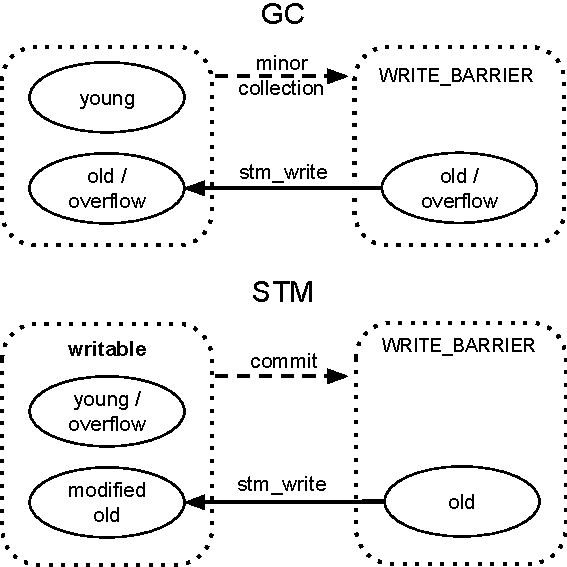
\includegraphics[width=0.8\columnwidth]{object_states.pdf}
  \caption{Object states handled by the write barrier\label{fig:obj_states}}
\end{figure}


\subsection{Write Barrier}

The job of the write barrier is twofold: it serves as a write barrier
for the garbage collector (GC) and the STM system. These two jobs are
depicted in Figure~\ref{fig:obj_states}. The GC needs to keep track of
objects that may contain references to young, movable objects. These
objects need to be traced during minor collections to update
references to moved objects. Young objects automatically get traced if
the GC ascertains that they survive the collection by being reachable
from traced objects. So far, this is how generational GCs generally
work. But the STM system also needs to record objects in the
write set, acquire write locks, and privatise their pages
(copy-on-write). It only needs to do this for old objects from
previous transactions, as any other object is not known to other
transactions anyway.

The \textbf{fast path} of the write barrier is very simple. We only
need to check for the flag \lstinline!WRITE_BARRIER! in the object's
header through its $SO$ and call the slow path if it is set. This flag
is set either if the object is old and comes from an earlier
transaction, or if there was a minor collection (in this case, the flag
is added again on all objects, including new overflow objects). The flag
is never set on young, freshly allocated objects. This fast path
covers all cases for the GC and for the STM system (see
Listing~\ref{lst:w_fast}).

\begin{code}[h]
\begin{lstlisting}
void stm_write(SO):
	if SO->flags & WRITE_BARRIER:
		write_slowpath(SO)
\end{lstlisting}
\caption{Write barrier fast path\label{lst:w_fast}}
\end{code}

\begin{code}[h]
\begin{lstlisting}
void write_slowpath(SO):
	// GC part:
	list_append(to_trace, SO)
	if is_overflow_obj(SO):
		SO->flags &= ~WRITE_BARRIER
		return
	// STM part
	stm_read(SO)
	lock_idx = SO >> 4
  retry:
	if write_locks[lock_idx] == our_num:
		// we already own it
	else if write_locks[lock_idx] == 0:
		if cmp_and_swap(&write_locks[lock_idx],
					    0, our_num):
			list_append(modified_old_objects, SO)
			privatize_pages(SO)
		else:
			goto retry
	else:
		w_w_contention_management()
		goto retry
	SO->flags &= ~WRITE_BARRIER
\end{lstlisting}

\caption{Slow path of the write barrier\label{lst:w_slow}}
\end{code}


The \textbf{slow path} is shown in Listing~\ref{lst:w_slow}.  For
each object, this code is called at most once between two minor collections.
First comes the \emph{GC part}: In any case, the object will be added
to the list of objects that need tracing in the next minor collection
(\lstinline!to_trace!). Any reference we write to this object will
be kept alive and up-to-date during minor collections.

The check for \lstinline!is_overflow_obj()! looks at the
\lstinline!overflow_number!  and tells us if the object was actually
created in this transaction. In that case, we do not need to execute
the following \emph{STM part}.  We especially do not need to privatise
its pages since no other transaction knows about these overflow
objects. Even if they reside in non-private pages, it is guaranteed
that no other transaction can have a reference to them.

Up to here, we see that all cases of the GC shown in
Figure~\ref{fig:obj_states} are handled. What is left is to handle the
cases of the STM system that need to make old objects writable.

For the \emph{STM part}, we first perform a read barrier on the
object. We then try to acquire its write lock. \lstinline!write_locks!
is a simple, \emph{global} array of bytes that is indexed with the
$SO$ of the object divided by 16. Note, ``global'' here really means
it is a single array with data for all segments, there is no address
translation going on to access its elements contrary to e.g.\ the
read markers array.  If we already own the lock, we are done.
If someone else owns the lock, we perform  write-write contention
management that aborts either us or the current owner of the
object.  If the lock is not owned so far, and if we succeed in
acquiring it using an atomic
\lstinline!cmp_and_swap!, we need to add the object to the write set
(a simple list called \lstinline!modified_old_objects!).  We then
privatise the page or pages where it resides (copy-on-write).

In all cases, we remove the \lstinline!WRITE_BARRIER!  flag from the
object before we return. Thus, we never trigger the slow path again
before we do the next minor collection or we start the next
transaction.\footnote{We always do a minor collection during a commit.}

Note that we have three kinds of objects: \emph{young, overflow} and
\emph{old} objects. Young and overflow objects were created in the
same transaction; old objects always come from previous transactions.
The close integration between STM and the GC allows us to use this
information effectively: young objects do not trigger the slow path at
all, overflow objects only need to be handled by the GC part of the
write barrier once between collections, and only the old objects need
to be handled by the STM part \emph{once per transaction}. The
privatisation step in particular is done very rarely because the pages
stay private until the next major collection where they may get
re-shared. This keeps the overhead of the write barrier very low in
the common cases.


\subsection{Abort}

Aborting a transaction is rather easy. The first step is to reset the
nursery and all associated data structures. The second step is to go
over all objects in the write set (\lstinline!modified_old_objects!)
and reset any modifications in our private pages by copying from the
sharing-segment. What is left is to use \lstinline!longjmp()!  to jump
back to the location initialised by a \lstinline!setjmp()!  in
\lstinline!stm_start_transaction()!.  Increasing the
\lstinline!read_version! for the next transaction is also done there.




\subsection{Commit}

Committing a transaction needs a bit more work. First, we synchronise
all threads so that the committing one is the only one running and all
the others are waiting in safe points.\footnote{This design choice is
important to support our very cheap barriers. It is a trade-off that
works best if the number of concurrent threads is small.
See section~\ref{subsub:sync} for how we mitigate the costs.}
We then go through the write
set (\lstinline!modified_old_objects!)  and check the corresponding
\lstinline!read_markers!  in other threads~/ segments. If we detect a
read-write conflict, we perform contention management to either abort us or
the other transaction, or to simply wait a bit (see Section~\ref{subsub:contentionmanagement}).

After verifying that there are no conflicts anymore, we copy all our
changes (i.e.\ objects in our write set) to all other segments,
including the sharing-segment. This is safe since we synchronised all
threads. We also need to push overflow objects generated by minor
collections to other segments, since they may reside partially in
private pages. At that point we also get a new
\lstinline!overflow_number! by increasing a global counter, so that it
stays globally unique for each transaction. Increasing the (local)
\lstinline!read_version!  is then done at the start of a new
transaction.


\subsection{Thread Synchronisation\label{subsub:sync}}

A requirement for performing a commit is to synchronise all threads so
that we can safely update objects in other segments. To make this
synchronisation fast and cheap, we do not want to insert an additional
check regularly to see if synchronisation is requested. We
use a trick relying on the fact that dynamic languages are usually
very high-level and thus allocate a lot of objects very regularly.
This is done through the function \lstinline!stm_allocate!  shown
in Listing~\ref{lst:alloc_func}.

\begin{code}[h]
\begin{lstlisting}
object_t *stm_allocate(ssize_t size_rounded):
    result = nursery_current
	nursery_current += size_rounded
	if nursery_current > nursery_end:
		return allocate_slowpath(size_rounded)
	return result
\end{lstlisting}
\caption{Function to allocate objects\label{lst:alloc_func}}
\end{code}

This code does simple bump-pointer allocation in the nursery. If there
is still space left in the nursery, we return
\lstinline!nursery_current!  and bump it up by
\lstinline!size_rounded!.  The interesting part is the check
\lstinline!nursery_current > nursery_end!  which will trigger the slow
path of the function to possibly perform a minor collection
to free up space in the nursery.

If we want to synchronise all threads, we can rely on this check being
performed regularly. So what we do is to set the
\lstinline!nursery_end!  to some small number in all segments that we
want to synchronise. The mentioned check will then fail in those
segments and call the slow path. In \lstinline!allocate_slowpath!
they can simply check for this condition and enter a safe point.

Note, this works well for interpreters that really allocate things
all the time. In the presence of an optimising just-in-time compiler,
some loops may indeed not allocate anything and therefore still need
the insertion of a safe-point check.

% For other synchronisation requirements, for example:
% \begin{itemize}[noitemsep]
% \item waiting for a segment to be released,
% \item waiting for a transaction to abort or commit,
% \item waiting for all threads to reach their safe points,
% \end{itemize}
% we use a set of condition variables to wait or signal other threads.


\subsection{Contention Management\label{subsub:contentionmanagement}}

On encountering conflicts, we employ contention management to solve
the problem as well as we can. The general rules are:

\begin{itemize}
\item prefer transactions that started earlier to younger transactions
  to increase the chance of long transactions succeeding
\item to support \emph{inevitable} transactions, we always prefer them
  to others since they cannot abort (similar to~\cite{blundell06})
\end{itemize}

We can either simply abort a transaction to let the other one succeed,
or we can also wait until the other transaction committed. The latter
is an interesting option if we are trying to commit a write and
another transaction already read the object. We can then signal the
other transaction to commit as soon as possible and wait. After
waiting, there is now no conflict between our write and the already
committed read anymore.



\section{Evaluation}

We evaluate our system in a Python interpreter called
PyPy and compare to CPython.
\begin{description}
\item[PyPy] (version 2.3) is an implementation of an
  interpreter for the Python language. It has a special focus on speed
  and provides a just-in-time (JIT) compiler to speed up applications
  running on top of it. We compare between normal PyPy
  using a GIL and a PyPy with STM. All code is available at~\cite{pypy}.
\item[CPython] (version 2.7.6) is the reference implementation of the Python
  language. It is the most widely used interpreter for this language.
  The implementation uses a GIL for synchronisation in multi-threaded
  execution and it does not feature a JIT compiler.
\end{description}

Here, we will not go into detail about the integration of our STM
system with PyPy's JIT. In fact, we will disable it for all benchmarks
except those in Section~\ref{subsec:jit-benchs}. The STM-JIT
integration is currently still incomplete and not tested much. The
JIT-less interpreter provides a much more consistent environment for
the STM system, so we remove some unknown variables by disabling it.
Furthermore, we think the interpreter-STM evaluation is more relevant
at this stage as the results can be more directly applied to other
similar interpreters. PyPy's JIT~\cite{cfbolz09}, however, is quite
unique as it is a JIT tracing the interpreter instead of the
interpreted language itself. This demands its own thorough
evaluation, which is out of the scope of this paper.


We performed all benchmarks on a machine with an Intel Core i7-4770
CPU~@3.40GHz (4 cores, 8 threads) with disabled Hyper-Threading and
Turbo Boost for less variation in the results.  There are 16~GiB of memory
available and we ran them under Ubuntu 14.04 with a Linux 3.13.0
kernel. The STM system was compiled with a number of segments $N=4$
and a maximum amount of memory of 1.5~GiB (both are configurable at
compile time).

For each point in the plots, we took 5 measurements and report the
arithmetic mean with the standard deviation as error bars. Average
speedup numbers are calculated using the geometric mean. For the JIT
benchmarks, we first let the JIT warm up by doing a few additional
iterations before the actual measurement.

% benchmarks with: pypy-c--Ojit-d1454093dd48+-14-05-26-17:16
% that's with stmgc 70c403598485

% Sometimes with JIT, sometimes without.
% For scaling & memory w/o jit, since the jit can optimize away
% many allocations and exposes the overhead more.

\subsection{Scaling}

To asses how well the STM system scales on its own (without any real
workload), we execute the loop in Listing~\ref{lst:scaling_workload}
on 1 to 4 threads on the PyPy interpreter with STM.

\begin{code}[h]
\begin{lstlisting}
def workload():
    i = 20000000
    while i:
        i -= 1
\end{lstlisting}
\caption{Dummy workload\label{lst:scaling_workload}}
\end{code}

For the results in Figure~\ref{fig:scaling}, we
normalised the average runtimes to the time it took on a single
thread. From this we see that there is additional overhead introduced
by each thread ($12.3\%$ for all 4 threads together). Every thread
adds some overhead because during a commit, there is one more thread
which has to reach a safe point. Additionally, conflict detection
needs to check for conflicts in all concurrently running transactions.

While not ideal, we think that $12.3\%$ is acceptable on four
threads. In terms of throughput, 4 threads have $3.54\times$
more iterations per second than a single thread.

\begin{figure}[h]
  \centering
  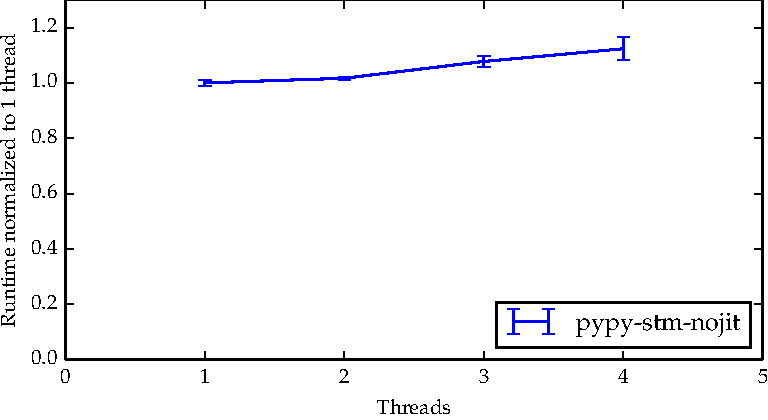
\includegraphics[width=1\columnwidth]{plots/scaling.pdf}
  \caption{Scalability of the STM system\label{fig:scaling}}
\end{figure}


\subsection{Small-Scale Benchmarks\label{sec:performance-bench}}

For the following sections we use a set of six small benchmarks
available at~\cite{pypybenchs}:

\begin{itemize}
\item \emph{btree} and \emph{skiplist}, which are both inserting,
  removing, and finding elements in a data structure from multiple
  threads
\item \emph{threadworms}, which simulates worms walking on a grid in
  parallel and checking for collisions with each other
\item \emph{mandelbrot}, \emph{raytrace}, and \emph{richards}, which
  all perform some independent computations in parallel (embarrassingly
  parallel)
\end{itemize}

We use atomic blocks to easily synchronise access to shared
data structures in the first three benchmarks. For the embarrassingly
parallel benchmarks, we do not need any explicit synchronisation at
all. These atomic blocks are simulated with a single global lock
when running on top of GIL-supported interpreters. With our STM
system, they map to transactions that will execute optimistically
in parallel.


%%% TODO: if time permits
% \subsection{Overhead Breakdown}

% \remi{do it on a non-jit build (see reason above)}
% \remi{gs:segment prefix overhead is virtually none (maybe instruction cache)}
% \remi{update numbers in pypy/TODO}

% \begin{itemize}
% \item time taken by read \& write barriers
% \item time spent committing \& aborting (maybe with different numbers
%   of threads; maybe split conflict detection and obj sync on commit)
% \item time in GC
% \end{itemize}





\subsection{Non-JIT Benchmarks}
First we run our benchmarks on three different interpreters: CPython
(GIL), PyPy with STM, and PyPy with the GIL (all without a JIT). The
results are shown in Figure~\ref{fig:performance-nojit}.

As expected, GIL-supported interpreters do not scale with the number
of threads. They even become slower because of the overhead of
thread-switching and GIL handling (see~\cite{beazley10} for a detailed
analysis).

PyPy using our STM system (\emph{pypy-stm-nojit}) scales in all
benchmarks to a certain degree. It scales best for the embarrassingly
parallel ones ($avg=2.6\times$ speedup) and a little less for
the others ($avg=2.0\times$ speedup). The reason for this difference is
that in the former group there are no real, logical conflicts -- all
threads do independent calculations. STM simply replaces the GIL in
those programs. In the latter group, the threads work on a common data
structure and therefore create much more conflicts, which limits the
scalability. Here we make active use of the STM-supported atomic
blocks to synchronise access to the data structure. The hope
is that the STM system is still able to parallelise, even if we use
the atomic blocks in a coarse-grained way. While less than the other
benchmarks, we indeed see some speedup going from 1 to 3 threads.
There is no visible benefit from 3 to 4 threads, even a slight
regression.

Looking at the average overhead from switching from GIL to STM, we see
that it is $\approx 43.3\%$. The maximum in richards is $71\%$. In all
benchmarks \emph{pypy-stm-nojit} beats \emph{pypy-nojit} already on
two threads despite of this overhead.  The achieved speedup comparing
STM to the GIL is between $1.14\times$ and $1.94\times$.

Still, STM rarely beats CPython's \emph{single-thread} performance. However, for
programs that need concurrency in CPython and that use threads to
achieve this, it also makes sense to look at the overhead induced by
the GIL on multiple threads. From this perspective, the STM
implementation beats CPython's performance in all but two benchmarks.

Since PyPy comes with a JIT~\cite{cfbolz09} to make its overhead
compared to CPython go away, we will now look at how well STM works
together with it.

\begin{figure}[h]
  \centering
  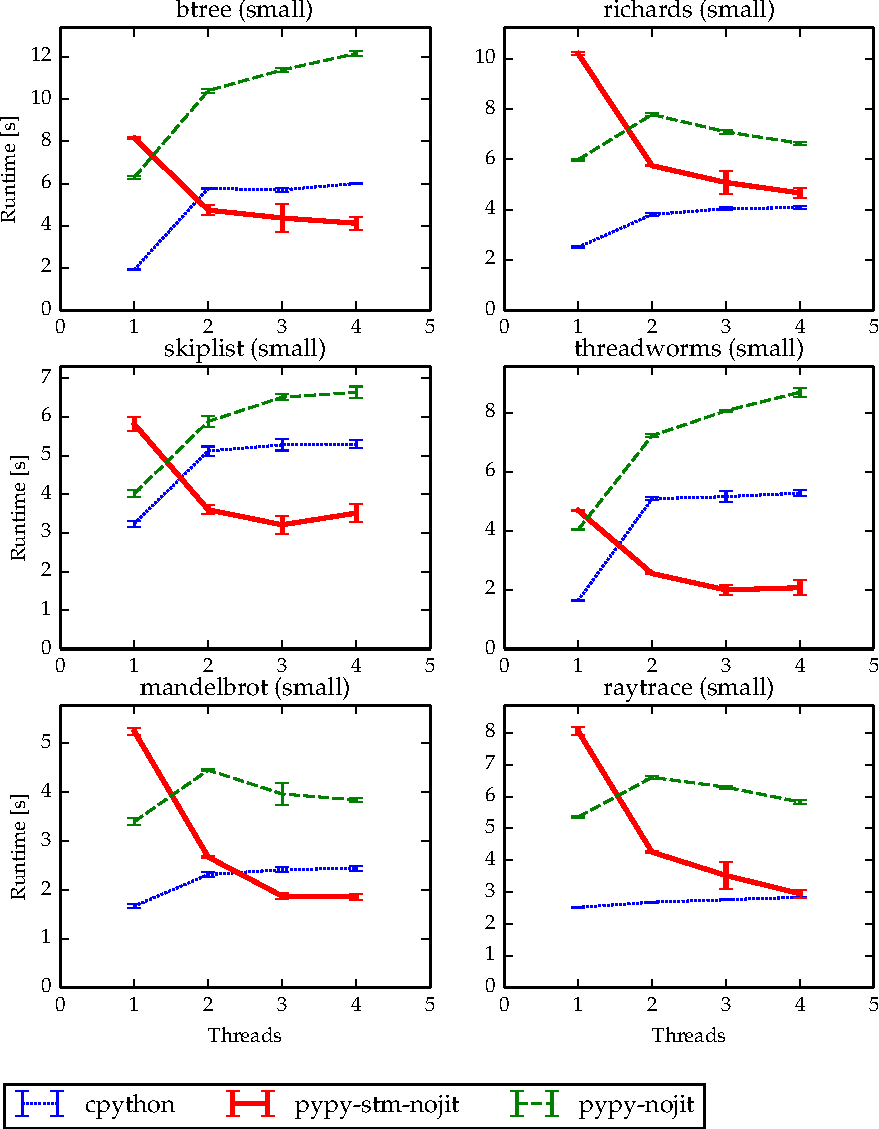
\includegraphics[width=1\columnwidth]{plots/performance_nojit.pdf}
  \caption{Comparing execution time between interpreters without a JIT
    and using small input sizes\label{fig:performance-nojit}}
\end{figure}



\subsection{JIT Benchmarks\label{subsec:jit-benchs}}

We would like to regard enabling the JIT as a simple performance
enhancement, but that is not what happens in reality. First, since the
JIT~\cite{cfbolz09} bases its decision of what to compile on runtime
profiling, running in multiple threads, it may compile different
things in each run because of the non-deterministic thread-scheduling
of the operating system (OS). Second, it is able to perform some
advanced optimisations. Because compilation is already non-deterministic,
so are these optimisations. And third, we did
not have enough time to optimise integration with STM so that the JIT
exposes the overhead of STM more by speeding up all the rest.
For these reasons, the following results have to be taken with a grain
of salt.

The speedups from enabling the JIT in these benchmarks range from
$10-50\times$. This is why we had to do without CPython here, since it
would be much further up in the plots. Also, to make jitting
code worthwhile, we increased the input size of all benchmarks to get
reasonable execution times (denoted with ``(large)'' in benchmark names).

We also ran these benchmarks on Jython\footnote{version
2.7b1~\cite{webjython}}, an implementation of Python on top of the
Java Virtual Machine (JVM).  Instead of a GIL, this interpreter uses
fine-grained locking for synchronisation. Even though it can use the
JVM's JIT compiler, its performance in these benchmarks is behind
PyPy's by a factor of $5-10\times$. Because of that it does not
make sense to include it in this evaluation. In the future, we would
like to do an extensive comparison between the STM approach and
fine-grained locking. It is out of the scope of this paper to do
this thoroughly.

The results are presented in Figure~\ref{fig:performance-jit}. We
see that the performance is much less stable. There is certainly more
work required in this area. The slowdown factor for switching from GIL
to STM ranges around $1-2.4\times$, and we beat GIL performance
in half of the benchmarks.

We see that generally, the group of embarrassingly parallel benchmarks
scales best. (There is a notable performance stability problem in the
\emph{richards} benchmark. This is a bug we will fix in the future.)
The other three benchmarks scale barely or not at all with the number of
threads. The reason for this is likely again the conflicts in the
latter group. Right now, because the code runs much more quickly with
the JIT than without, it has the effect of making the transactions
logically longer.  This increases the
likelihood of conflicts between them and therefore limits scalability
even more than in the no-JIT benchmarks.

Overall, PyPy without STM is around $2\times$ slower than CPython.
Enabling its JIT allows it to outperform CPython by a huge margin.
We see the same kind of speedup on PyPy with STM when enabling the
JIT. This means that STM does not generally inhibit the JIT from
optimising the programs execution, which is already a very important
result on its own. We also see that for some
benchmarks, STM is already able to give additional speedups
compared to just the JIT-induced acceleration. This looks very
promising and investigating when this is not the case is the next
logical step.


\begin{figure}[h]
  \centering
  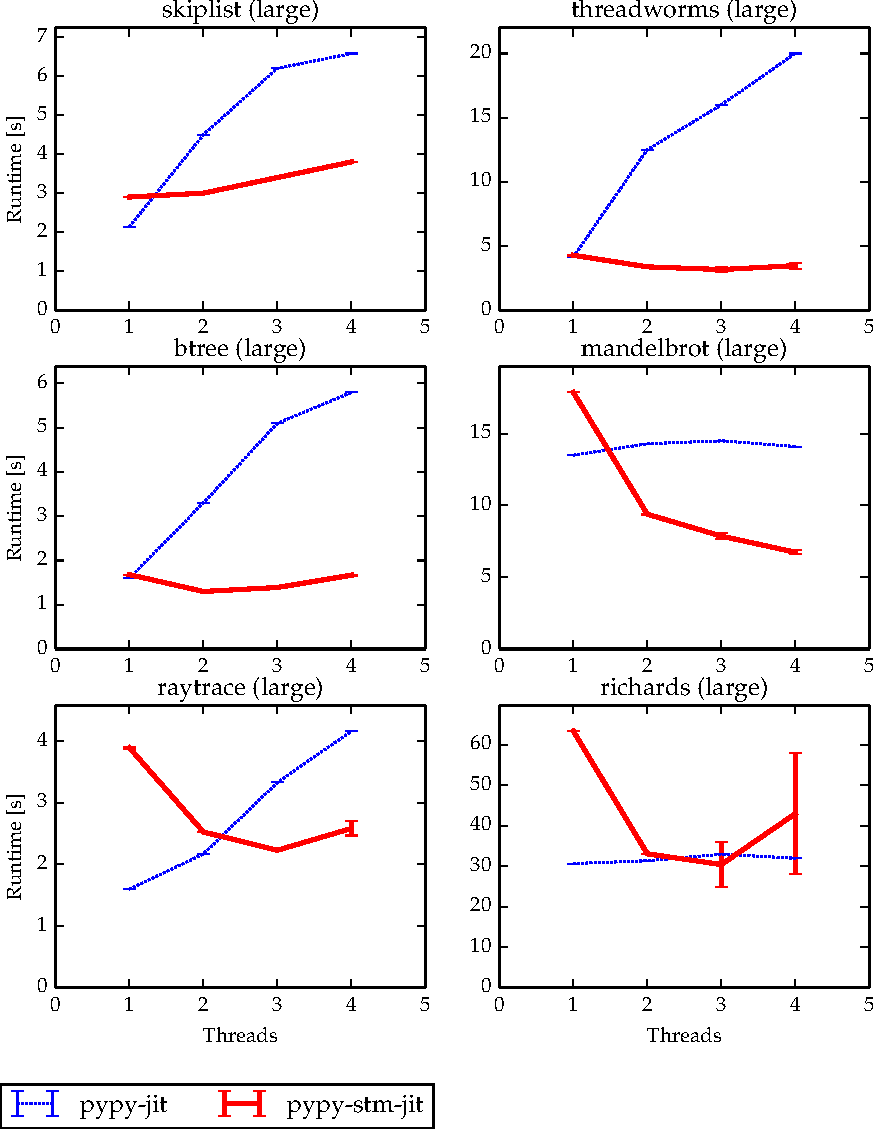
\includegraphics[width=1\columnwidth]{plots/performance.pdf}
  \caption{Comparing execution time between interpreters with JIT
    and large input sizes\label{fig:performance-jit}}
\end{figure}



\section{Related Work}

There have been several attempts at removing the GIL using TM. We
ourselves did a few earlier attempts with more conventional STM
systems~\cite{stmupdate13}. Because of the huge overhead we
encountered, the result was mostly useless on $\le 4$ CPU cores.
Since this could be considered the main operating conditions of
dynamic languages, it was never as useful as we wanted it to be.

Other attempts using HTM~\cite{nicholas06,odaira14,fuad10} show
promising results, especially the very recent~\cite{odaira14} that
examines the current generation of Intel CPUs. However, they did a
simplification by essentially disabling the GC during the
benchmarks. This may be valid for the hand-tuned allocations in their
interpreter. For us the GC is essential, and because it is a moving
GC, it unfortunately touches a lot more memory and thereby reaches the
HTM capacity much faster.  This, and the fact that HTM's capacity
limits do not allow the implementation of arbitrary-sized atomic blocks, let
us to believe that STM is the right choice at the moment.

There are multiple attempts at removing the limits of HTM by means of
\emph{virtualising} HTM~\cite{rajwar05,chung06}. Indeed this may also
be the future direction of our research. So far, some of them depend
on additional hardware features. Or in the case of~\cite{chung06},
they have the assumption that most transactions fit the HTM capacity
and that virtualisation is only a fallback. Our use case, however,
features arbitrarily long transactions, which is why this assumption
first has to be verified again in this setting.

From the other end, there also have been attempts at lowering the
overhead of STM~\cite{warmhoff13,spear09} especially for a low number
of CPU cores. \cite{spear09} works well for some workloads, in the
case of a dynamic language VM, however, we have to assume any possible
workload.  \cite{warmhoff13} uses a compile-time approach to select
from multiple optimised STMs. Their partitioned FastLane STM seems to
provide good performance already on two threads using master and
helper threads. It would be interesting to see if its design also
performs well in our use case.

Similarly to us, \cite{martin09} use memory management techniques to
provide isolation between transactions. They focus on providing strong
atomicity between transactional and non-transactional code.  We,
however, use inevitable transactions to provide strong atomicity
for non-reversible operations and otherwise do not have to deal
with non-transactional code.  Additionally, while they use page fault
handlers to detect conflicts, we use traditional write barriers. There
are only some superficial similarities between the approach presented
here and theirs.


% Similar STMs:
% \begin{itemize}
% \item FastLane: \cite{warmhoff13}
% \item TML: \cite{spear09}
% \item Virtualizing HTM: \cite{rajwar05}
% \item Page-based virtualizing HyTM: \cite{chung06}: page-level conflict
%   detection, otherwise hardware extensions required; assumes most
%   transactions fit HTM capacities (not so true here); COW using page-faults;
%   they assume OS-level access to page-tables (maybe not inherent to their
%   design); eval on simulator; value-based confl detection;

%  (XTM can be
%   implemented either in the OS as part of the virtual memory manager or
%   between underlying TM systems and the OS, like virtual machines;
%   Conflicts for overflowed transactions are tracked at page granularity;
%   XTM-e allows conflict detection at cache line granu-
%   larity, even for overflowed data in virtual memory)
% \item using mmap(): Memory-Mapped Transactions
% \item mem-protected conflict detection: \cite{martin09}
% \end{itemize}


\section{Conclusions}

% review of paper
As multi-core processors continue to increase the number of cores per
processor, it is important that dynamic languages like Python embrace
parallelism.  We report here an effort to replace the Global
Interpreter Lock (GIL) used in many Python implementations with
transactional memory (TM). The key factor for success is a close
integration of a software TM (STM) and the garbage collector to
provide atomicity, synchronisation, and memory management in a unified
way.  The STM system supports atomic blocks as a user abstraction and
thereby provides a scalable synchronisation mechanism to Python
applications.


% STM needs good performance:
The solution presented here is based on a software TM system developed
as an independent and reusable C library for integration in dynamic
language interpreters. As the 
STM is a vital part of the interpreter, good performance is
essential. We present an interesting way to combine the existing
memory segmentation and virtual memory features of current CPUs to
lower the overhead of STM. This software implementation reduces
dramatically the cost of transactional memory and at the same time
provides an opportunity to integrate the STM system with garbage
collection.  This implementation leverages the processor's memory
segmentation hardware, which has lately not received much attention.
Unfortunately, processor architects seem to
undervalue this hardware resource -- in the evolution from the x86 to
the x86{-}64 architecture, 4 out of 6 segment registers have been
removed. This development potentially threatens the STM strategy
outlined here and we want to remind the architecture community that
this unit can support interesting implementations -- a viewpoint that
has also been expressed by other researchers (see also
\cite{bennet10}).

% results, outlook
The early results presented here are very encouraging. STM as a simple
GIL replacement scales well and yields an average speedup of $2.6\times$ for
embarrassingly parallel workloads on 4 threads.  When also used for
synchronisation in the form of atomic blocks, the average speedup
still reaches $2.0\times$.

To generally outperform the best-performing Python systems (Jython,
PyPy), integration of the STM-based approach with a JIT compiler is
necessary. Our early results of this integration suggest that there is
no inherent incompatibility between STM and PyPy's JIT.  Once the
implementation matures, the approach outlined here serves not only as a
simple GIL replacement but also provides a way forward towards a
parallel programming model for Python.

%% \appendix
%% \section{Appendix Title}

%% This is the text of the appendix, if you need one.

\acks
We would like to thank the following people for their valuable
input and the many fruitful discussions: Carl F. Bolz, Michael Faes,
Pascal Felber, Maciej Fijalkowski, Patrick Marlier, and Aristeidis Mastoras.

% We recommend abbrvnat bibliography style.

\bibliographystyle{abbrvnat}

% The bibliography should be embedded for final submission.



\begin{thebibliography}{}
\softraggedright

\bibitem{cfbolz09} Carl Friedrich Bolz, Antonio Cuni, Maciej
  Fijalkowski, and Armin Rigo. 2009. Tracing the meta-level: PyPy's
  tracing JIT compiler.  \emph{In Proceedings of the 4th workshop on the
    Implementation, Compilation, Optimization of Object-Oriented Languages
    and Programming Systems} (ICOOOLPS '09).

\bibitem{kevin10} Kevin Millikin, Florian Schneider. 2010.  A New
  Crankshaft for V8.
  \url{http://blog.chromium.org/2010/12/new-crankshaft-for-v8.html}

\bibitem{ionmonkey} IonMonkey from Mozilla. 2014.
  \url{https://wiki.mozilla.org/IonMonkey/Overview}

\bibitem{wayforward14} Remigius Meier, Armin Rigo. 2014. A Way Forward
  in Parallelising Dynamic Languages. To appear in ICOOOLPS'14.

\bibitem{cpython} CPython. \url{www.python.org}
\bibitem{webjython} The Jython Project, \url{www.jython.org}
\bibitem{ironpython} IronPython. \url{www.ironpython.net}
\bibitem{pypy} PyPy Project. \url{www.pypy.org}

\bibitem{beazley10} Beazley, David. "Understanding the Python GIL."
  \emph{PyCON Python Conference}. Atlanta, Georgia. 2010.

\bibitem{harris10} Harris, Tim, James Larus, and Ravi
  Rajwar. "Transactional memory." \emph{Synthesis Lectures on Computer
  Architecture 5.1} (2010)

\bibitem{guerraoui08}
  Rachid Guerraoui and Michal Kapalka. 2008. On the correctness of
  transactional memory. In \emph{Proceedings of the 13th ACM SIGPLAN
    Symposium on Principles and practice of parallel programming} (PPoPP
  '08).

\bibitem{blundell06} Blundell, Colin, E. Christopher Lewis, and Milo
  Martin. "Unrestricted transactional memory: Supporting I/O and system
  calls within transactions." (2006).

\bibitem{spear08} Michael F. Spear and Michael Silverman and Luke
  Daless and Maged M. Michael and Michael L. Scott. 2008. "Implementing
  and exploiting inevitability in software transactional memory."  In
  \emph{Proc. 37th IEEE international conference on parallel
    processing} (ICPP '08), 59-66

\bibitem{fergus02} Fergus Henderson. 2002. Accurate garbage collection
  in an uncooperative environment. \emph{In Proceedings of the 3rd
    international symposium on Memory management} (ISMM '02).

\bibitem{stmupdate13} Armin Rigo, Remigius Meier. 2013. Update on
  STM. \url{morepypy.blogspot.ch/2013/10/update-on-stm.html}

\bibitem{rajwar05} Ravi Rajwar, Maurice Herlihy, and Konrad
  Lai. 2005. Virtualizing Transactional Memory. In \emph{Proceedings of
    the 32nd annual international symposium on Computer Architecture}
  (ISCA '05).

\bibitem{chung06} JaeWoong Chung, Chi Cao Minh, Austen McDonald,
  Travis Skare, Hassan Chafi, Brian D. Carlstrom, Christos Kozyrakis,
  and Kunle Olukotun. 2006. Tradeoffs in transactional memory
  virtualization. \emph{SIGOPS Oper. Syst. Rev.} 40, 5 (October 2006),
  371-381.

\bibitem{martin09} Martín Abadi, Tim Harris, and Mojtaba
  Mehrara. 2009. Transactional memory with strong atomicity using
  off-the-shelf memory protection hardware. \emph{SIGPLAN Not.} 44, 4
  (February 2009), 185-196.

\bibitem{pypybenchs} PyPy benchmarks repository. 2014. Revision
  a26f2fb58413. \url{bitbucket.org/pypy/benchmarks}


%%%%%%%%%%%%%%%%%%%%%%%%%%%%%%%%%%%%%%%%%%%%%%%%%%%%%%%%%%%%

% \bibitem{dan07}
%   Dan Grossman. 2007. The transactional memory / garbage collection
%   analogy. \emph{In Proceedings of the 22nd annual ACM SIGPLAN
%     conference on Object-oriented programming systems and
%     applications} (OOPSLA '07).


\bibitem{odaira14}
  Rei Odaira, Jose G. Castanos, and Hisanobu Tomari. 2014. Eliminating
  global interpreter locks in Ruby through hardware transactional
  memory. In \emph{Proc. 19th ACM SIGPLAN Symposium on
    Principles and Practice of Parallel Programming} (PPoPP '14).

\bibitem{warmhoff13}
  Jons-Tobias Wamhoff, Christof Fetzer, Pascal Felber, Etienne Rivière,
  and Gilles Muller. 2013. FastLane: improving performance of software
  transactional memory for low thread counts. \emph{SIGPLAN Not.} 48, 8
  (February 2013), 113-122.

\bibitem{drago11} Aleksandar Dragojević, Pascal Felber, Vincent
  Gramoli, and Rachid Guerraoui. 2011. Why STM can be more than a
  research toy. \emph{Commun. ACM} 54, 4 (April 2011), 70-77.

\bibitem{cascaval08}
  Calin Cascaval, Colin Blundell, Maged Michael, Harold W. Cain, Peng
  Wu, Stefanie Chiras, and Siddhartha Chatterjee. 2008. Software
  transactional memory: why is it only a research
  toy?. \emph{Commun. ACM} 51, 11 (November 2008), 40-46.

\bibitem{nicholas06}
  Nicholas Riley and Craig Zilles. 2006. Hardware transactional memory
  support for lightweight dynamic language evolution. \emph{In
    Companion to the 21st ACM SIGPLAN symposium on Object-oriented
    programming systems, languages, and applications} (OOPSLA
  '06).

\bibitem{fuad10}
  Fuad Tabba. 2010. Adding concurrency in Python using a commercial
  processor's hardware transactional memory support. \emph{SIGARCH
  Comput. Archit. News 38}, 5 (April 2010), 12-19.

\bibitem{felber07}
  Pascal Felber and Torvald Riegel and Christof Fetzer and Martin
  Süßkraut and Ulrich Müller and Heiko Sturzrehm. 2007. Transactifying
  applications using an open compiler framework. \emph{TRANSACT}, August
  (2007): 4-6.

% \bibitem{bill06}
%   Bill McCloskey, Feng Zhou, David Gay, and Eric
%   Brewer. 2006. Autolocker: synchronization inference for atomic
%   sections. \emph{In Conference record of the 33rd ACM SIGPLAN-SIGACT
%   symposium on Principles of programming languages (POPL '06)}. ACM,
%   New York, NY, USA

\bibitem{spear09}
  Luke Dalessandro, Dave Dice, Michael Scott, Nir Shavit, and Michael
  Spear. 2010. Transactional mutex locks. In \emph{Proceedings of the
    16th international Euro-Par conference on Parallel processing: Part
    II} (Euro-Par'10), Pasqua D'Ambra, Mario Guarracino, and Domenico
  Talia (Eds.). Springer-Verlag, Berlin, Heidelberg, 2-13.

\bibitem{lamport79}
  L. Lamport. 1979. How to Make a Multiprocessor Computer That Correctly
  Executes Multiprocess Programs. \emph{IEEE Trans. Comput.} 28, 9
  (September 1979), 690-691.

\bibitem{victor11}
  Victor Pankratius and Ali-Reza Adl-Tabatabai. 2011. A study of
  transactional memory vs. locks in practice. In \emph{Proc.
     twenty-third annual ACM Symposium on Parallelism in Algorithms
    and Architectures} (SPAA '11).

\bibitem{christopher10}
  Christopher J. Rossbach, Owen S. Hofmann, and Emmett
  Witchel. 2010. Is transactional programming actually
  easier?. \emph{Proc. 15th ACM SIGPLAN Symposium on
    Principles and Practice of Parallel Programming} (PPoPP '10).


\bibitem{tim03}
  Tim Harris and Keir Fraser. 2003. Language support for lightweight
  transactions. \emph{In Proceedings of the 18th annual ACM SIGPLAN
    conference on Object-oriented programing, systems, languages, and
    applications} (OOPSLA '03), 388-402.

\bibitem{tim05} Tim Harris, Simon Marlow, Simon Peyton Jones, and
  Maurice Herlihy. 2008. Composable memory transactions.
  \emph{Commun. ACM} 51, 8 (August 2008), 91-100.


\bibitem{shan08}
  Shan Lu, Soyeon Park, Eunsoo Seo, and Yuanyuan Zhou. 2008. Learning
  from mistakes: a comprehensive study on real world concurrency bug
  characteristics. \emph{SIGARCH Comput. Archit. News} 36, 1 (March 2008),
  329-339.

\bibitem{bennet10}
  Bennet Yee, David Sehr, Gregory Dardyk, J. Bradley Chen, Robert
  Muth, Tavis Ormandy, Shiki Okasaka, Neha Narula, and Nicholas
  Fullagar. 2010. Native Client: a sandbox for portable, untrusted x86
  native code. \emph{Commun. ACM} 53, 1 (January 2010), 91-99.

% \bibitem{leis14}
%   Leis, Viktor, Alfons Kemper, and Thomas Neumann. "Exploiting
%   Hardware Transactional Memory in Main-Memory Databases."
%   \emph{Proc. of ICDE}. 2014.

% \bibitem{biased}
%   Kenneth Russell and David Detlefs. 2006. Eliminating
%   synchronization-related atomic operations with biased locking and
%   bulk rebiasing. \emph{In Proceedings of the 21st annual ACM SIGPLAN
%     conference on Object-oriented programing, systems, languages, and
%     applications} (OOPSLA '06).

\end{thebibliography}


\end{document}
